\begin{figure}[htpb]
    \centering\capstart{}
    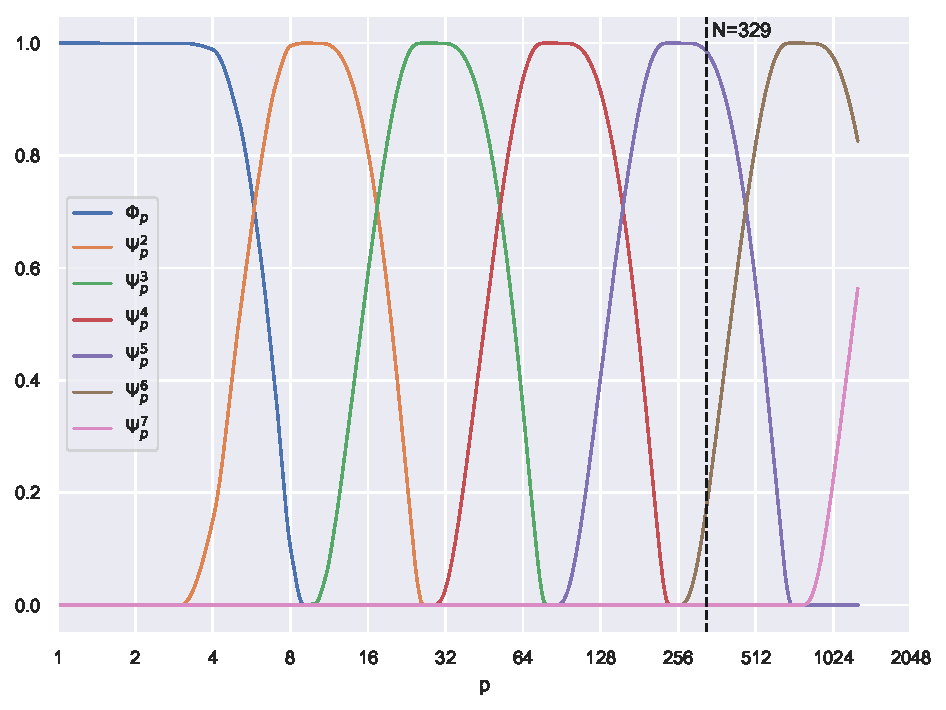
\includegraphics[width=\textwidth]{homer_slepian_tiling_b1275.pdf}
    \caption[
        The tiling of the Slepian line for the Homer head region
    ]{
        The tiling of the Slepian line with parameters \(\lambda=3\) and \(J_{0}=2\) with \(\imax=\num{1275}\) basis functions.
        The black dashed line marks the Shannon number for the Homer head region \(N=329\).
        The scaling function and the first five wavelets are non-zero, as the coefficients are within the Shannon number.
    }\label{fig:chapter5_tiling}
\end{figure}
